\documentclass{article}
\usepackage[T1]{fontenc}
\usepackage[right=1cm, left=1cm, top=1cm, bottom=2cm]{geometry}
\usepackage{parskip}
\usepackage{circuitikz}
\usepackage{pdflscape}
\usepackage{listings}
\usepackage{mathtools}
\usepackage{relsize}
\usepackage{graphicx}
\usepackage{float}
\usepackage{pgfplots}\pgfplotsset{compat = 1.18}

\title{Software Enginnering Fall 2023-2024 \\ VALUNI Design Specifications}
\author{  
Hussein Heggi 	\and
Ahmed Waseem Raslan 	\and
Sarah Elsamanody 	\and
Nour Abdalla 	\and
Youssef Elmahdy	\and
Ahmed Elbarbary	\and 
Ahmed Jaheen}
\usepackage{titling}
\renewcommand\maketitlehooka{\null\mbox{}\vfill}
\renewcommand\maketitlehookd{\vfill\null}  

\begin{document}

\begin{titlingpage}
\maketitle
\end{titlingpage}

\break

\tableofcontents

\break 


\section{Project Proposal}
\quad VALUNI is a platform where students have the opportunity to share their experiences and exchange knowledge and feedback regarding both professors and courses.  It would play a vital role in helping students hold sufficient knowledge that could ease up the process of choosing classes and preparing for exams. Our objective is to create a safe, dependable and organized environment that allows students to express their opinions in an honest and respectful way. We aim to motivate students when rating or writing their reviews through anonymity, and at the same time having certain guidelines that must be followed when using VALUNI. This will not only assist students, but also the overall University community including diverse facilities and professors. 

\subsection{Usage}
$\bullet$ Search for professors and courses feedback.  

$\bullet$ Rate professors on a variety of criteria which are explanation, fairness, organization, leniency, and accessibility.

$\bullet$ Rate courses based on difficulty level, workload, and learning outcomes.

$\bullet$ Course Evaluations per semester for universities to measure the educational quality.

\subsection{Risks} 

\subsubsection{Community Risks}
$\bullet$ \textbf{Defamation:} Students may post false or misleading reviews of professors, which could damage the professor's reputation and career.

$\bullet$ \textbf{Bias:} Student ratings of professors may be biased. For example, distinct students may go through different experiences such as receiving undesired grades , influencing the integrity of their ratings.

$\bullet$ \textbf{Increased Reliance on student feedback:} Professors may rely too heavily on student feedback for validation, which could negatively impact their teaching style. In addition, students may depend on the review itself without actually giving the professor a chance.

\subsubsection{Development Risks} 

$\bullet$ The website is not liked by its main target audience as well as not being used by the student body which will defeat the whole purpose of the website.

$\bullet$ The website is not perfectly secured which can lead to privacy issues and data breaches.

$\bullet$ The cost of developing and maintaining the website could be high which could result in problems with financial sustainability.

$\bullet$ The website may not be well-received by professors which can make the website unsuccessful.



\subsection{Motivation} 

\quad Nowadays, the majority of students find it difficult to navigate the right path when it comes to making decisions during their registration periods. It is a well known hustle amongst students as continuously trying  to find the suitable courses and professors that fits their best interest is a challenge.  In fact, some students initiated solving this problem by creating  RateAUCProfessors, a FaceBook group, to provide reviews about Professors and pass on evaluations to next colleagues. Eventually, some of the group members started posting content that is out of context which made it lose its academic focus. Not to mention, the data keeps increasing each semester which makes it difficult for students to search in an efficient way. Therefore, we came up with VALUNI  where our main purpose is to constantly and effectively serve the educational community. This is because it would incorporate not only accessible reviews on courses and professors but also help collect evaluations at the end of each semester; aiding the university to adopt rightful and recent evaluations regarding each aspect of the overall educational level. 

\break

\subsection{MVP Requirements (Requirements to be Implemented)}

	\quad User authentication (login etc)

	\quad User data encryption

	\quad Rating Courses

	\quad Rating Professors

	\quad Writing out a review with Rating

	\quad Parameterized Rating

	\quad Filtered Search on parameters	

	\quad Editing Reviews



\section{Requirements Specifications}

\subsection{Product Backlog}

\subsubsection{Functional Requirements}

	\quad User authentication 
	\vspace{-0.2cm}

	\qquad \scriptsize User login and verification that user is a university student \normalsize

	\quad Rating Courses

	\quad Rating Professors

	\quad Writing out a review with Rating
	\vspace{-0.2cm}

	\qquad \scriptsize When Reviewing students have the option to write a review with the parameterized rating \normalsize

	\quad Parameterized Rating
	\vspace{-0.2cm}

	\qquad \scriptsize Students can rate professors and courses on different parameters, such as workload, leniency \normalsize

	\quad Filtered Search on parameters 
	\vspace{-0.2cm}

	\qquad \scriptsize Students can filter out result or search for courses and professors based on parameters \normalsize

	\quad Reporting reviews

	\quad Editing Reviews

	\quad Admin ( university ) access to review data 
	\vspace{-0.2cm} 

	\qquad \scriptsize University can access critical semster review analytics as well as overall analytics \normalsize

	\quad Search for courses 

	\quad Search for professors 



\subsubsection{Non Functional Requirements} 

	\quad Fluid, Simple UI

	\quad Secure

	\quad Auto removing profanity on reviews

	\quad Prevent Review Bombing

	\quad Anonymous

	\quad Customer Service ( for universities )

	\quad Performance

	\quad Scalability

\subsection{Use Case Diagram} 

\begin{center}
	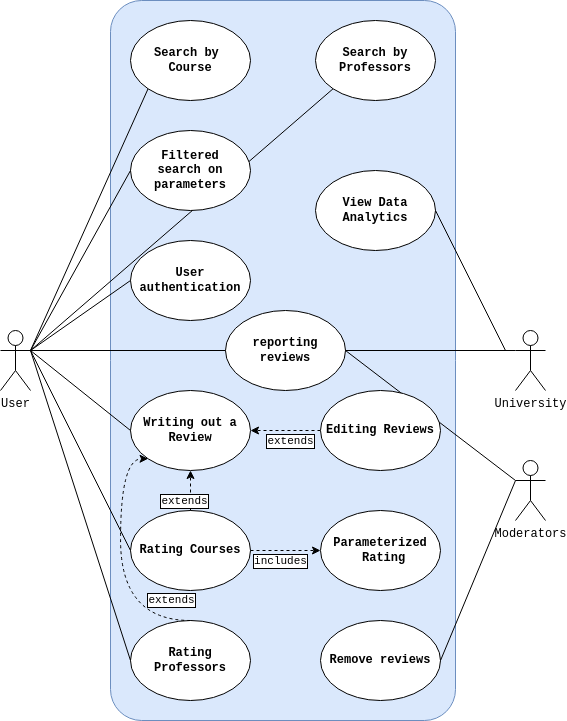
\includegraphics[scale=0.5]{../../Milestone_1/requirements_specification/USECASE.drawio.png}	
\end{center}

%use case narratives 


\subsection{Use Case Narratives}

\textbf{Use Case \#1: }
	
\quad \textbf{Title: User Authentication}

\quad\textbf{Use Case Description:}
Authentication during login to ensure the existence of the user account.
	
\quad\textbf{Primary Actor:} User
	
\quad\textbf{Secondary Actor:} Firebase
	
\quad\textbf{Pre-Condition:} User must have an account.
	
\quad\textbf{Textual Description:} 

\begin{center}
  \begin{tabular}{|c|c|c|} 
    \hline
    step & actor & direction \\  \hline
    1&User&Opens website \\ 
    2 & 
    Client & 
Provides Username \& Password Field for Users. \\
    3 & 
    User & 
Enters Valid Username \& Password \\
    4 & 
    Firebase & 
    Verify Username \& Password  \\
    5 &
    User &
    Logs in Successfully \& Views Homepage \\ \hline

  \end{tabular}
\end{center}


\textbf{Alternative Flows:}\\
3. User username \& password are not valid as user does not exist ; redirect or recommend signing up instead.\\
4. User username or password are invalid ; ask user to re-enter.

\textbf{Post-Conditions: }\\
User is authenticated and can access the app, homepage and its features. \\

\hrule

\textbf{Use Case \#2: }

\quad\textbf{Title:} Search by Course

\quad\textbf{Use Case Description:}
Users can navigate through the website by searching over courses.  Users use the search bar for desired courses to check its reviews or review it.

\quad\textbf{Primary Actor:} User

\quad\textbf{Secondary Actor:} Database access layer

\quad\textbf{Pre-Condition:} User already logged in and has authentication done. Courses must exist in the database system to be found in search.

\quad\textbf{Textual Description:}


\begin{center}
  \begin{tabular}{|c|c|c|} 
    \hline
    step & actor & direction \\  \hline

    1 & 
    User&
Clicking on Search Menu \\
    2 & 
    User & 
Writes the name of course \\
    3 & 
    Data access layer &
Searches for course \\
    4 & 
    Data access layer &
Returns Course \\
    5 & 
    Client  &
Course is viewed \\ \hline

  \end{tabular}
\end{center}

\textbf{Alternative Flows:}\\
	1-User can pick directly from the homepage the course he desires.\\
	2-If course is not found, nothing will be displayed.\\
\textbf{Post-Conditions:}\\
	Users now have the desired course, they can choose to either read or write a review.\\

\hrule 


\textbf{Use Case \#3: }

\quad \textbf{Title:} Filtered Search on Parameters

\quad\textbf{Use Case Description:} User filters the parameters they require when viewing reviews

\quad\textbf{Primary Actor:} Data access layer

\quad\textbf{Secondary Actor:} Client

\quad\textbf{Pre-Condition:} User exists in order to access the settings and adjust his parameters
	Textual Description:


\begin{center}
  \begin{tabular}{|c|c|c|} 
    \hline
    step & actor & direction \\  \hline

    1 & 
    User & 
    Go to settings  \\ 
    2 & 
    User & 
Choose adjust parameters \\
    3 & 
    Data access layer &
Removes the unwanted parameters \\
    4 &
    User  &
Confirms and can go back \\
 \hline



  \end{tabular}
\end{center}

\textbf{Alternative Flows:}
	User did not confirm his changes, leaving his parametrized ratings unchanged.

  \textbf{Post-Conditions: }
User has confirmed his preferred parameters to view. \\

\hrule 


\textbf{Use Case \#4: }

\quad\textbf{Title}: Writing Out a Review

\quad\textbf{Use Case Description:}  Users can choose/instructor a course to write a review about

\quad\textbf{Primary Actor:} User

\quad\textbf{Secondary} Actor: Data access layer

\quad\textbf{Pre-Condition: }
User successfully logs in as in this use case he is only choosing what to write a review about.

\quad\textbf{Textual Description:}


\begin{center}
  \begin{tabular}{|c|c|c|} 
    \hline
    Step &
    Actor&
Description \\ \hline
    1 &
    User &
Clicking on Search Menu \\
    2 &
    User &
Writes the name of course \\
    3 &
    Data access layer &
Searches for course/instructor \\
    4 &
    Data access layer &
Returns course/instructor \\
    5 &
    User &
Chooses course/instructor \\ \hline

\end{tabular}
\end{center}

\textbf{Alternative Flows:}\\
	Choose course/instructor from homepage, and add the review.\\
  \textbf{Post-Conditions:}\\
Users found the course/instructor they were looking to write a review about. \\


\hrule 



\textbf{Use Case \#5: }
	Title: Rating Courses

Use Case Description:. He also has two options for writing reviews, rating only or adding a detailed review as well. 

	Primary Actor:User

	Secondary Actor: Data access layer

	oPre-Condition: User must have taken the course beforehand.
	Textual Description:



\begin{center}
  \begin{tabular}{|c|c|c|}
\hline
Step &
Actor &
Description\\ \hline
1 &
Client &
Gives options for writing a review \\

2 &

User & 
Chooses option  \\
3& 
Client &
Field for writing only or writing and rating  \\
4& 
User &
Writes in field given and confirms \\ \hline

\end{tabular}
\end{center}

	Alternative Flows:\\
	Choose the course from the homepage, and add the review.\\
	Post-Conditions:\\
	Users successfully added their review on the course.\\

  \hrule

Use Case \#6: 

	Title: Rating Professors

Use Case Description: Users can choose an instructor to write a review about. He also has two options for writing reviews, rating only or adding a detailed review as well. 
	Primary Actor:User

	Secondary Actor: Data access layer

	Pre-Condition: User must have taken the course with the instructor beforehand.

	Textual Description: 
	
\begin{center}
  \begin{tabular}{|c|c|c|}
    \hline
    Step & 
    Actor & 
Description \\ \hline
    1 &
    Client &
Gives options for writing a review \\
    2 &
    User & 
Choses option \\
    3&
    Client&
Field for writing only or writing and rating\\ 
    4 &
    User &
Writes in field given and confirms \\ \hline
\end{tabular} 
\end{center}

Alternative Flows:\\
	Choose the instructor from the homepage, and add the review.\\
	Post-Conditions:\\
	Users successfully added their review on the course.\\ 

\hrule 



Use Case \#7: 

	Title: Search by Professors

	Use Case Description:
Users can navigate through the website by searching over courses which include professors.  Users use the search bar for desired professors to check its reviews or review it.

	Primary Actor: User

	Secondary Actor: Database access layer

Pre-Condition: User already logged in and has authentication done. Instructors must exist in the database system to be found in search.

	Textual Description:





\begin{center}
  \begin{tabular}{|c|c|c|}
    \hline
    Step & 
    Actor & 
Description \\ \hline 

    1 & 
    User &
Clicking on Search Menu \\
    2 &
    User &
Writes the name of course \\
    3 &
    Data access layer &
Searches for instructor \\
    4 &
    Data access layer &
Returns instructor \\
    5 &
    Client  &
Instructor is viewed \\ \hline


  \end{tabular} 
\end{center}


Use Case 8: 

	Title: View Data Analytics

	Use Case Description: University has access to view the data in the database.

	Primary Actor: University

	Secondary Actor: Database

Pre-Condition: There exists data in the database for the University to have access to.

	Textual Description:


\begin{center}
  \begin{tabular} {|c|c|c|}
    \hline
    Step&
    Actor&
Description \\ \hline
    1&
    University &
Requesting data \\
    2&
    Data access layer &
Fetch required data\\ 
    3&
    Database &
Search required data \\
    4 &
    Data access layer &
Return formatted data \\ \hline


  \end{tabular} 
\end{center}

Alternative Flows:\\
	No alternative flow\\
	Post-Conditions:\\
University successfully has access to the database.\\

\hrule 

Use Case \#9: 

	Title: Editing Reviews

	Use Case Description: User can open his posted reviews and edit the content.

	Primary Actor: User

	Secondary Actor: Data access layer

	Pre-Condition: User has already written the review to be edited.

	Textual Description:


\begin{center}
\begin{tabular}{|c|c|c|}
  \hline
  Step & 
  Actor & 
Description \\ \hline
  1 & 
  User &
Check for post history \\
  2 &
  User &
Choses review \\
  3 &
  User &
Edits review \\
  4 &
  User &
Confirms  \\
  5 &
  Data access layer &
Updates changes made \\  \hline
\end{tabular} 
\end{center}

Post-Conditions:\\ 
Users edited their desired reviews. \\
Alternative Flows:\\
	User forgets to confirm, so changes are not saved.\\
	Alternative Flows Post-Conditions: \\
	User review is not edited. \\

  \hrule

Use Case \#10: 

	Title: Parameterized Rating

  Use Case Description: A Rating based on multiple parameters, each parameter contributes to overall rating of professors/courses. User gets to Rate professors/courses based on these parameters.
	
  Primary Actor: User
	
  Secondary Actor: Data Access Layer
	
  Pre-Condition: The User must have\\
				A. taken a course with the professor ( professor review ) OR\\
				B. taken the course in the current semester 		AND\\
				C. User has not reviewed professor/course prior
	
        Textual Description:

\begin{center} 
\begin{tabular}{|c|c|c|}
\hline
Step &
Actor &
Description \\ \hline
1 &
User &
Fills Rating Form \\
2&
Data Access Layer&
Sends Rating to DB\\
3&
Database&
Stores rating \\ \hline
\end{tabular}
\end{center} 

Use Case \#11: 

	Title: Remove Reviews

	Use Case Description: Ability to Remove reviews (Moderator Privilege) 

	Primary Actor: Moderator

	Secondary Actor: Database

	Pre-Condition: Review is present

	Textual Description:

\begin{center} 
\begin{tabular}{|c|c|c|}
  \hline
  Step &
  Actor &
Description \\ \hline
  1&
  Moderator &
Delete Review \\
  2 &
  Data Access Layer &
Signal deleted Review \\
  3&
  Database &
Remove review \\ \hline
\end{tabular}
\end{center}

Alternative Flows: No alternative flow\\
	Post-Conditions: The Review is deleted\\

\hrule

Use Case \#12: 

	Title: Reporting Reviews

Use Case Description: User can optionally report reviews they deem inappropriate.

	Primary Actor: Client

	Secondary Actor: Moderators

	Pre-Condition: There is a review to report.

	Textual Description:

\begin{center}
\begin{tabular}{|c|c|c|}
  \hline
  Step &
  Actor&
Description \\ \hline
  1&
  User&
Initiate report\\
  2&
  Data Access Layer&
File the report \\
  3&
  Moderator&
Review the report\\
  4&
  Moderator&
Delete Review\\ \hline

\end{tabular}
\end{center}

Post-Conditions: \\
	Review is deleted from the database and is updated on the client side.\\
Alternative Flows:\\
	4- Moderator, Dismiss report\\
	Alternative Flow Post-Conditions:\\
	Review is not deleted\\


\break
\section{Design Specifications}
\subsection{High Level Architecture}  
\begin{center}
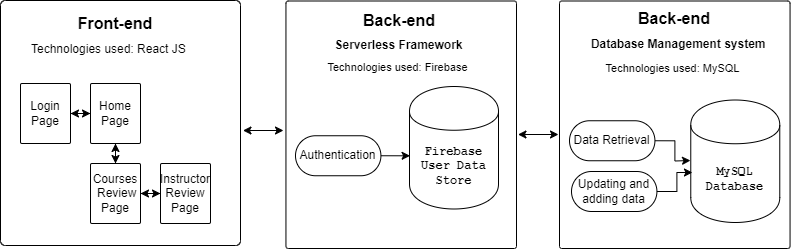
\includegraphics[scale=0.65]{../../Milestone_2/Diagrams/High_Level_Arch.png}
\end{center}
\quad Front-end is implemented using React JS where it is used to implement the login, home, results, and review pages. The authentication of users is done through firebase, a server-less framework, where it contains a database including the email addresses and passwords of the university students. The user's data which is previewed on the web app is accessed through a database on a local host which is managed and manipulated by MySQL workbench. The SQL database includes all necessary information that is needed for Valuni and it is updated whenever a user adds a new review. Lastly, the frontend and backend are connected together using Node js. 
 
\subsection{Detailed Level Architecture: Monolithic Layered Architecture} 
\begin{center}
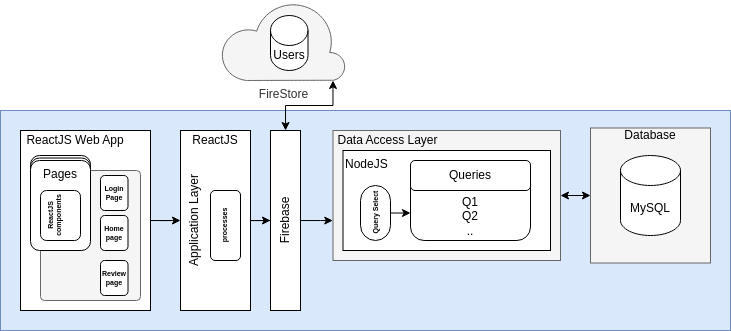
\includegraphics[scale=0.65]{../Diagrams/MonolithicArch.png}
\end{center}

\quad Monolithic architecture is suitable to represent the architecture of the Web app ,Valuni, as this project is not divided into subsystems, but rather the components are interconnected with one another. Therefore, the data being transferred continuously goes through diverse stages and technologies to reach the end-user. This diagram shows a clear path and flow of the Valuni architecture where the web app is built and linked with firebase through ReactJs. After the authentication process is done by firebase, the input is processed by the data access layers using queries which are manipulated and linked through the MySQL database that contains all the necessary data needed by the web application.

\subsection{Activity Diagrams}  

Valuni’s main functionalities revolve around two main activities which are writing or reading reviews. Therefore we decided to represent each process through a diagram.  

\subsubsection{Writing Reviews} 

\begin{center}
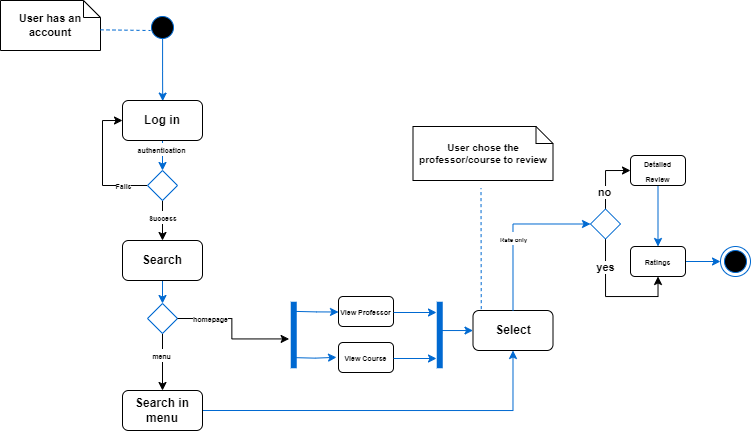
\includegraphics[scale=0.65]{../Diagrams/WritingReview_Activity.png}
\end{center}

\quad This visual representation illustrates the internal processes involved in achieving a key function, specifically the process of writing reviews. It begins with user authentication upon login, if it succeeds it goes on by offering two search options: directly through the homepage or the search menu. If the user does the search and selection  directly from the homepage, they would have professors and courses as two simultaneous choices. After they choose, they can either rate and write a detailed review or rate only. 

\subsubsection{Reading Reviews}


\begin{center}
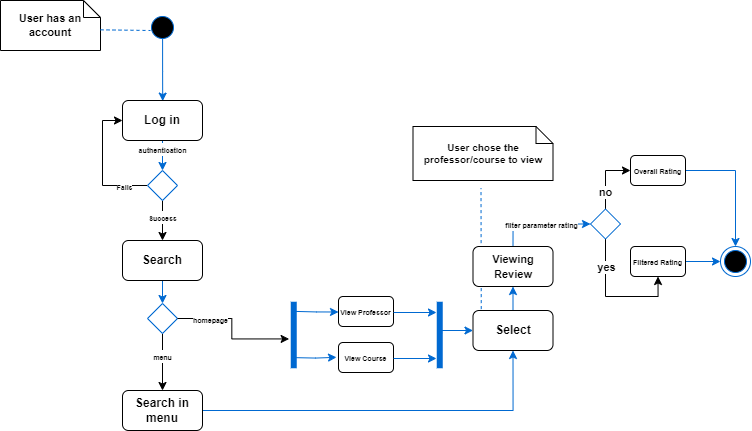
\includegraphics[scale=0.65]{../Diagrams/ReadingReview_Activity.png} 
\end{center}

\quad The second key option, reading reviews, is dynamically portrayed through this activity diagram where it begins with the same sequence as the previous diagram. However, after selecting the course or professor, the user views the detailed review, if it exists, followed by either the overall rating or the filtered rating, depending on their choice.


\subsection{MVC: Model View Controller Model} 

\begin{center} 
  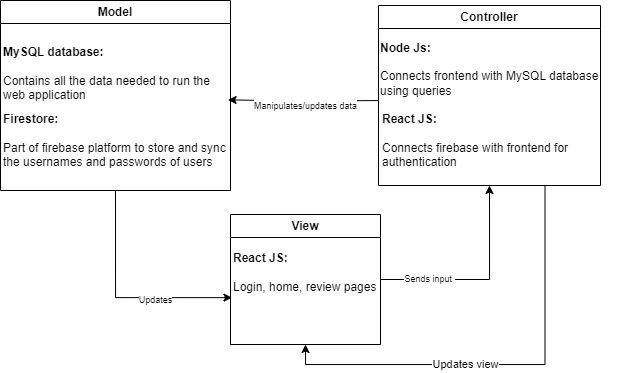
\includegraphics[scale=0.65]{../Diagrams/MVC.png}
\end{center}

\quad Since Valuni has a number of technologies used, it was crucial to add a design pattern to help in visualizing how our functionalities work and communicate behind the scenes. The model consists of the two main data structures used to store, update, and sync data which are MySQL databases along with Firestore. The content within these structures aid in the updating of the view of the application itself through the different GUIs presented by Valuni. The functionalities within the diverse web pages send input to the controller, processing and filtering it to reach the required output through the data access layer needed to update the view. On the other hand, the input sent may need some manipulation which is why it could be sent to the model to retrieve the needed data and finally it gets updated. 

\subsection{Class Diagram}  

\begin{center}
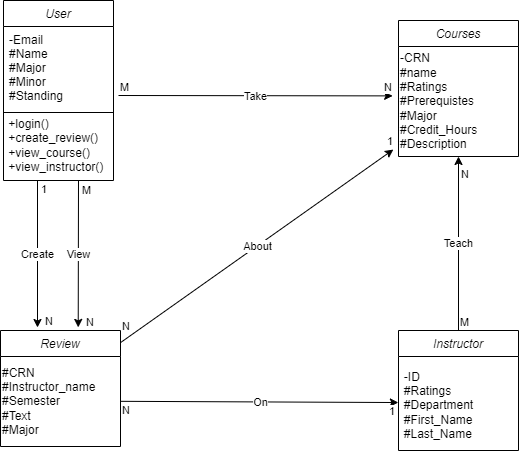
\includegraphics[scale=0.8]{../../Milestone_2/Diagrams/ClassDiagram.png} 
\end{center}

\quad As a starting point, it was decided to implement four main classes: users, courses, review, and instructors. Each of these classes represent one of the tables from the database and are interconnected with each other. Since the user is the only one who can access the web app along with changing the database, its class is the only one containing methods. The rest of the classes contain the attributes which describe them as they do not affect the functionalities of the software. 


\subsection{Sequence Diagram} 
\begin{center}
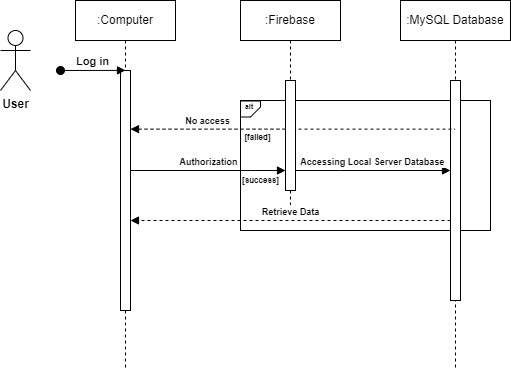
\includegraphics[scale=0.8]{../../Milestone_2/Diagrams/SequenceDiagram.png} 
\end{center} 

\quad This sequence diagram portrays the connection between the system interfaces used by Valuni. The user starts by logging in and the authentication is done via firebase which is a serverless framework. If the user exits, the needed data will be retrieved from the database which is managed by MySQL workbench and reflected on the GUI of Valuni. On the other hand, if the authentication fails there will be no access to the database containing the user’s information.

\subsection{State Diagram} 
\begin{center}
    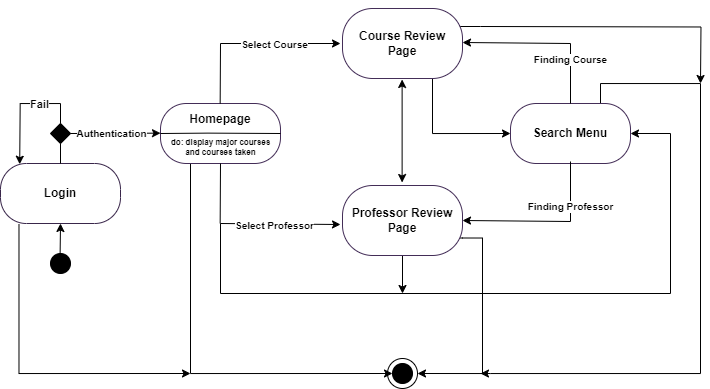
\includegraphics[scale=0.7]{../../Milestone_2/Diagrams/B&W_StateDiagram.png}    
\end{center} 

\quad Valuni has four web pages, login, home, course review, and professor review page. This diagram is a representation of the dynamic behind the transition between different web pages, where each arrow describes how to transform from one page to another. Since the web application could be closed from any page, all pages are connected to the end point. 

\subsection{Entity Relationship Diagram}  
\begin{center}
    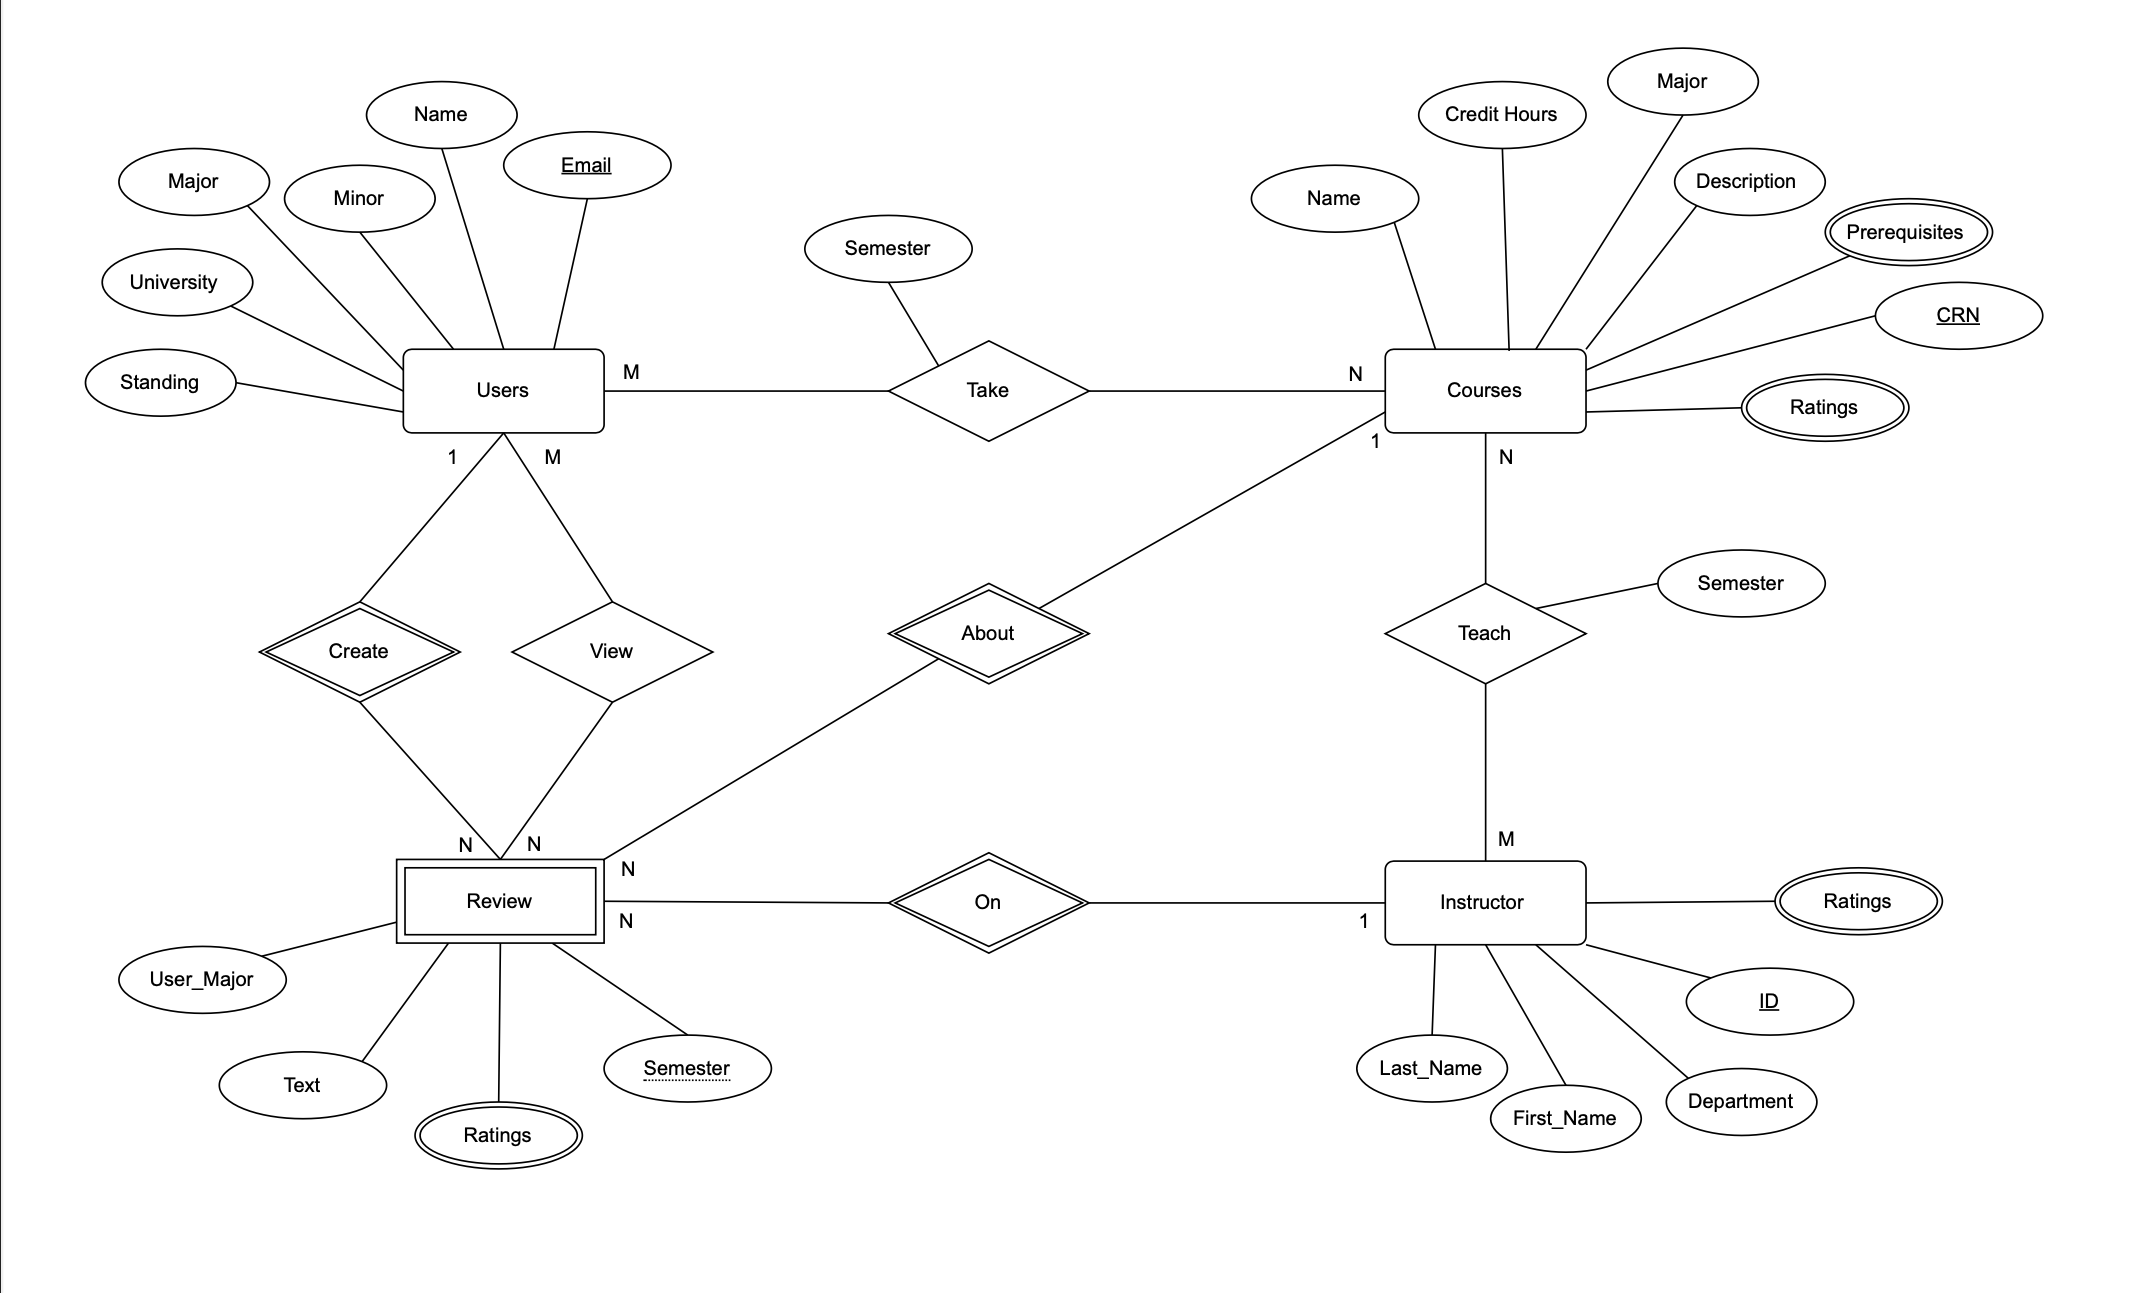
\includegraphics[scale=0.55]{../../Milestone_2/Diagrams/VALUNI_ERD.png}    
\end{center} 

\quad The ERD graphically represents and depicts the structural organization of entities, their attributes, and relationships within a database system. Strong entities in our database are users, courses, and instructors, which possess distinct attributes and play vital roles in the Valuni database schema. On the other hand, review is a weak entity as it lacks an independent key for unique identification, depending on the existence of other entities. This is because a review can not exist without users creating them about either courses or instructors. 
\break 

\newgeometry{left=0.5cm, bottom=0.5cm, top=0.5cm, right=0.5cm}
\begin{landscape}

\section{Second Sprint Retrospective} 

\subsection{Sprint log} 
\scriptsize

\begin{tabular}{llll}
Title &
  URL &
  Assignees &
  Status \\
Masking firebase API keys &
  https://github.com/Ahmed-Waseem77/valuni/issues/25 &
  Ahmed-Waseem77, elbarbary, mego74 &
  In Progress \\
Valuni Presentation &
  https://github.com/Ahmed-Waseem77/valuni/issues/7 &
  nouryasser1, SamanodyJr &
  Done \\
Search drop down menu &
  https://github.com/Ahmed-Waseem77/valuni/issues/37 &
  SamanodyJr, youssef-S-Elmahdy &
  In Progress \\
Review box component &
  https://github.com/Ahmed-Waseem77/valuni/issues/41 &
  youssef-S-Elmahdy &
  Done \\
Review page button &
  https://github.com/Ahmed-Waseem77/valuni/issues/42 &
  youssef-S-Elmahdy &
  Done \\
Finishing DB SQL schema &
  https://github.com/Ahmed-Waseem77/valuni/issues/38 &
  Hussein-Heggi, nouryasser1 &
  Done \\
Finishing up NodeJS API &
  https://github.com/Ahmed-Waseem77/valuni/issues/40 &
  Ahmed-Waseem77, elbarbary, mego74 &
  Done \\
generating some mock up data &
  https://github.com/Ahmed-Waseem77/valuni/issues/39 &
  Hussein-Heggi, nouryasser1 &
  Done \\
Review Page &
  https://github.com/Ahmed-Waseem77/valuni/issues/36 &
  SamanodyJr, youssef-S-Elmahdy &
  Done \\
Documentation Diagrams for various methodologies &
  https://github.com/Ahmed-Waseem77/valuni/issues/27 &
  nouryasser1 &
  Done \\
Connect the application to the local server database &
  https://github.com/Ahmed-Waseem77/valuni/issues/4 &
  Hussein-Heggi, nouryasser1 &
  Done \\
Creating the SQL Database on the local server &
  https://github.com/Ahmed-Waseem77/valuni/issues/22 &
  Hussein-Heggi, nouryasser1 &
  Done \\
Database schema design &
  https://github.com/Ahmed-Waseem77/valuni/issues/8 &
  elbarbary, Hussein-Heggi, mego74, nouryasser1 &
  Done \\
Home Page/ Landing page &
  https://github.com/Ahmed-Waseem77/valuni/issues/35 &
  Ahmed-Waseem77, SamanodyJr, youssef-S-Elmahdy &
  Done \\
Merging Backed functionalities and resolving resulting conflicts &
  https://github.com/Ahmed-Waseem77/valuni/pull/30 &
  Ahmed-Waseem77 &
  Done \\
Dev f update &
  https://github.com/Ahmed-Waseem77/valuni/pull/43 &
  Ahmed-Waseem77 &
  Done
\end{tabular}

\normalsize  

The primary objective for this sprint is almost finishing the front-end where the functionalities built will be completely operational, yet not linked to the mock up data. In addition, alongside is a fully operational login system, all seamlessly connected to the database. Lastly, the backend would contain almost all the data and queries needed to connect and link the rest of the webpages to it in the next sprint. 



\begin{center} 
  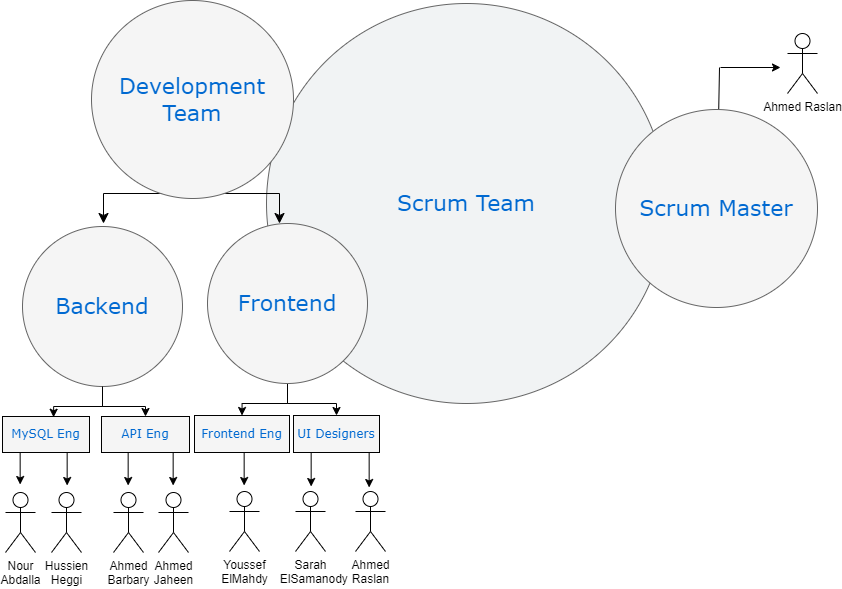
\includegraphics[scale=0.35]{"../../Milestone_2/Diagrams/ScrumTeam.png"}
\end{center}

\subsection{SCRUM team organization}  

\quad In the development of Valuni, the team was divided into two parts: frontend and backend. When each team started working on their tasks, it was decided that the teams should be further divided to implement the idea of pair programming, working in a more effective and efficient way. Each sub-team had their own tasks and responsibilities which were all merged together at the end of the sprint. The scrum master, Ahmed Raslan, continuously communicated with both ends of the team to ensure that everything was in place. 

\subsection{Pair Programming}
\quad Most of the Tasks were done in pairs to increase cooperation between teams. Even found ourselves having 3 team members working together in some rare cases. This made our team more aware of the code and the hurdles we are facing.



\end{landscape} 
\restoregeometry.


\subsection{Sprint Review}
Understimation of the complexity of linking multiple frameworks together and getting them to work was a key hurdle in our progress. Moving on, we should measure the level of competence of our developers witht the amount of time we have.  

For the next sprint our main focus is to develop the MVP to a deployable state.

\end{document}

